\documentclass{sigchi}
% \usepackage{titlesec}
% Use this section to set the ACM copyright statement (e.g. for
% preprints).  Consult the conference website for the camera-ready
% copyright statement.

% Copyright
\CopyrightYear{2021}
%\setcopyright{acmcopyright}
\setcopyright{acmlicensed}
%\setcopyright{rightsretained}
%\setcopyright{usgov}
%\setcopyright{usgovmixed}
%\setcopyright{cagov}
%\setcopyright{cagovmixed}
% DOI
\doi{https://doi.org/10.1145/3313831.XXXXXXX}
% ISBN
\isbn{978-1-4503-6708-0/21/05}
%Conference
\conferenceinfo{CHI'21,}{May  25--30, 2021, Honolulu, HI, USA}
%Price
\acmPrice{\$15.00}

% Load basic packages
\usepackage{balance}       % to better equalize the last page
\usepackage{graphics}      % for EPS, load graphicx instead 
\usepackage[T1]{fontenc}   % for umlauts and other diaeresis
\usepackage{txfonts}
\usepackage{mathptmx}
\usepackage[pdflang={en-US},pdftex]{hyperref}
\usepackage{color}
\usepackage{booktabs}
\usepackage{textcomp}

% Some optional stuff you might like/need.
\usepackage{microtype}        % Improved Tracking and Kerning
% \usepackage[all]{hypcap}    % Fixes bug in hyperref caption linking
\usepackage{ccicons}          % Cite your images correctly!
% \usepackage[utf8]{inputenc} % for a UTF8 editor only

\usepackage{todonotes}

% Paper metadata (use plain text, for PDF inclusion and later
% re-using, if desired).  Use \emtpyauthor when submitting for review
% so you remain anonymous.
\def\plaintitle{Towards Eco-Friendly, Efficient \& Effective Edge-Device Neural Machine Translation}
\def\plainauthor{First Author}
\def\emptyauthor{}
\def\plainkeywords{Neural Machine Translation; Mobile Devices; Open Neural Network Exchange; Edge Computing; Attention}
\def\plaingeneralterms{Documentation, Standardization}

% llt: Define a global style for URLs, rather that the default one
\makeatletter
\def\url@leostyle{%
  \@ifundefined{selectfont}{
    \def\UrlFont{\sf}
  }{
    \def\UrlFont{\small\bf\ttfamily}
  }}
\makeatother
\urlstyle{leo}

% To make various LaTeX processors do the right thing with page size.
\def\pprw{8.5in}
\def\pprh{11in}
\special{papersize=\pprw,\pprh}
\setlength{\paperwidth}{\pprw}
\setlength{\paperheight}{\pprh}
\setlength{\pdfpagewidth}{\pprw}
\setlength{\pdfpageheight}{\pprh}


\definecolor{linkColor}{RGB}{6,125,233}
\hypersetup{%
  pdftitle={\plaintitle},
% Use \plainauthor for final version.
%  pdfauthor={\plainauthor},
  pdfauthor={\emptyauthor},
  pdfkeywords={\plainkeywords},
  pdfdisplaydoctitle=true, % For Accessibility
  bookmarksnumbered,
  pdfstartview={FitH},
  colorlinks,
  citecolor=black,
  filecolor=black,
  linkcolor=black,
  urlcolor=linkColor,
  breaklinks=true,
  hypertexnames=false
}
\setlength{\parindent}{5ex}


\begin{document}

\title{\plaintitle}

\numberofauthors{1}
\author{%
  \alignauthor{Dane Williamson\\
    \affaddr{University of Virginia (UVA)}\\
    \affaddr{Charlottesville, VA}\\
    \email{dw3zn@virginia.edu}}\\
}

\maketitle


\begin{abstract}
    UPDATED---\today. This paper seeks to outline the economic, environmental and computational costs associated with Neural Translation Models (NMT) within Cyber-Physical Systems (CPS) and the Internet of Things (IoT). While these costs are too vast and numerous to be immediately resolved within this paper, a precedent is set for augmented development and deployment pipelines to reduce the computational costs and carbon footprint of ML Inference by performing computation on models stored on Edge Computing (EC) Devices.
\end{abstract}


% ACM Classfication

\begin{CCSXML}
<ccs2012>
   <concept>
       <concept_id>10003120.10003138.10003139.10010906</concept_id>
       <concept_desc>Human-centered computing~Ambient intelligence</concept_desc>
       <concept_significance>100</concept_significance>
       </concept>
   <concept>
       <concept_id>10010147.10010178.10010179.10010180</concept_id>
       <concept_desc>Computing methodologies~Machine translation</concept_desc>
       <concept_significance>500</concept_significance>
       </concept>
   <concept>
       <concept_id>10002944.10011122.10002947</concept_id>
       <concept_desc>General and reference~General conference proceedings</concept_desc>
       <concept_significance>100</concept_significance>
       </concept>
   <concept>
       <concept_id>10010583.10010662.10010673</concept_id>
       <concept_desc>Hardware~Impact on the environment</concept_desc>
       <concept_significance>300</concept_significance>
       </concept>
 </ccs2012>
\end{CCSXML}

\ccsdesc[100]{Human-centered computing~Ambient intelligence}
\ccsdesc[500]{Computing methodologies~Machine translation}
\ccsdesc[100]{General and reference~General conference proceedings}
\ccsdesc[300]{Hardware~Impact on the environment}

% Author Keywords
\keywords{\plainkeywords}

% Print the classification codes
\printccsdesc
% Please use the 2012 Classifiers and see this link to embed them in the text: \url{https://dl.acm.org/ccs/ccs_flat.cfm}



\section{Introduction}
\par Training state-of-the art Neural Machine Translation (NMT) models on modern datasets is often computationally expensive. Even with the usage of multiple computers with Graphics Processing Units (GPUs), the training process can take days. The model produced is typically of the order of several Gigabytes (GB) in size and is thus unsuitable for usage on a typical EC device as the typical EC device has only a few GB of storage. The Switch Transformer model (Switch-C) \cite{switch} for example, has approximately over a trillion parameters and is trained on a 745 GB dataset. The Switch transformer holds record results on multiple Natural Language Processing (NLP) benchmarks. Cyber-Physical systems which are interactive with humans will no doubt be unable to provide the resources required to support such a model. Thusly, inference is typically offloaded to a cloud device which can provide these resources. This offloading introduces additional latency and entirely negates the effectiveness of devices when network connectivity is less than optimal or entirely compromised or unavailable.

\par NMT has achieved stellar performance in large-scale, high-resource environments. Since these resources are typically unavailable in the pocket of an average user or inside the average IoT device and the need for translation is ever more required in a diverse and increasingly connected world, in this paper a compromise is sought for model resources and translation accuracy. Using various modern techniques and frameworks  a proof of concept for a low resource, computationally inexpensive, high accuracy NMT model for deployment on edge-computing devices is provided.

\par The contributions made in this paper are as follows:

\begin{itemize}
  \item The need for considering the financial and environmental impact of computationally expensive machine learning architectures is demonstrated.
  \item A precedent is provided for ensuring that computationally expensive models can be deployed on less computationally powerful devices for Cyber Physical Systems and the Internet of Things.
  \item  The carbon footprint of inferences made by a Neural Machine translation system is reduced by ensuring inference can be performed without the utilization of cloud resources. 
\end{itemize}

The utility of these contributions is demonstrated by performing an NMT task of converting English to French.

\section{Background and Motivation} 
\par NMT may potentially address the shortcomings of traditional machine translation systems, such as Statistical Machine Translation (SMT), due to its ability to directly learn the associations between an input text and output text.  Despite the merits of NMT, it still has inherent deficiencies such as slow training times, slow inference speed and fragility to rare or out of vocabulary words. For deployment on resource-constrained edge devices, NMT models are entirely unsuited. Modern translation systems such as google translate are ubiquitously available to users with an internet connection. However in situations where translation is required but connectivity is limited, this is inconvenient. Interactive Cyber-Physical Systems should be well-equipped to be responsive to a user regardless of his or her language of choice. To address this issue the deployment of pre-trained models on mobile devices is proposed. The inference time and memory occupancy of these models is not suitable for immediate deployment on typical edge devices. However model compression can reduce the memory occupancy and inference time of these devices and render them more efficient.

\subsection {Natural Language Processing in Cyber-Physical Systems and the Internet of Things}
\par A Cyber-Physical system may be formally defined as a system that combines the capabilities of computing, communications and data storage to monitor or control entities in the physical world. \cite{cpssurvey} Recent research in the field of CPS has seen application of NLP techniques to optimize human-in-the-loop CPS. In \cite{cityresolver} researchers leverage Language Modeling techniques for extracting Signal Temporal Logic (STL) specifications for smart cities. In \cite{cpsbots} researchers leverage NLP for integration in home automation using chat bots.

\par In an increasingly interconnected and nomadic world, society is communicating at an unprecedented rate. Interactive CPS will no doubt be required to interface with individuals from a variety of linguistic backgrounds. The additional overhead of performing translational inference on cloud devices will degrade the performance of these interactive CPS. Furthermore the cloud-based operations will create a broader attack surface to compromise these systems. The work proposed here therefore seeks to provide a compromise for computationally inexpensive edge-based NMT for Interactive CPS.

\par The aforementioned desire for Edge-Device based Inference in Interactive CPS and AI-enabled IoT devices is an area of research that has recently received attention. In the forthcoming IoT revolution, there will no doubt be various sources of network latency and bottleneck as devices seek to utilize network bandwidth. In \cite{edgeml}, the researchers seek to pave the way to the "Internet of Conscious Things" by reviewing the main techniques for executing ML inference on low-performance hardware. A noteworthy finding in \cite{edgeml} is that Neural Network based machine learning typically requires less computational power in deployment than in training. For ML inference in the Internet of Conscious Things, \cite{edgeml} propose several solutions such as lightweight model design, model compression and optimal edge computing hardware. In light of these proposed solutions, the nature of the typical NLP model must be considered before a solution for deployment on edge devices can be synthesized.

\subsection{Resource Consumption}
Modern NLP has seen an abundance of language models which involve a large number of parameters and training data. \cite{stochasticparrots} The advent of modern deep-learning systems has not come without a significant trade-off between model performance and environmental impact. Recent research has been focused in conflicting and opposite directions, i.e. a line of research has been focused on building relatively large models with many parameters designed for computationally complex tasks, see Table \ref{tab:modeltable}. By contrast other researchers have aimed to build models which are more computationally efficient. In \cite{systematic}, the researchers propose online leaderboards to motivate and incentivize research in energy efficient and computationally effective machine learning (ML) models. As stated by \cite{systematic} a major roadblock to a comprehensive understanding of the potential climate impacts of ML research is a lack of resources to track the realtime energy consumption and carbon emissions associated with ML research and work particularly in fueling modern tensor processing hardware. 

\par While researchers such as \cite{systematic} seek to establish a centralised framework for reporting the carbon impact of ML research, others such as \cite{energypolicy} seek to estimate the financial and environmental costs of training successful modern neural network architectures. In fact, an astounding claim made in \cite{energypolicy} is that the model emissions from training the popular transformer, BERT \cite{bert} are roughly equivalent to a those of a trans-American flight. To achieve marginally higher state-of-the-art Bilingual Evaluation Understudy (BLEU) \cite{bleu} scores, researchers potentially incur several hundreds of thousands of dollars worth of cost in computation power and produce non-trivial carbon emissions. As if to underscore this issue, Strubel et al \cite{energypolicy} implore the NLP community to prioritize the development of efficient models and hardware. 

\par The issue of excessive resource requirements for NLP models on resource constrained edge devices is clearly illustrated. In \cite{nnembedded}, a system for compressing deep neural networks for sensing applications on embedded devices is developed, called DeepIoT.
In following the precedent set by DeepIot, a framework for compressing deep neural networks for NMT on edge devices is developed here. Whereas the researchers in \cite{edgeml} developed a novel algorithm for compression, the popular compression method of quantization is used here. The framework produced can be visualised in Figure \ref{fig:nmtedge}.


\begin{figure}[t]
\centering
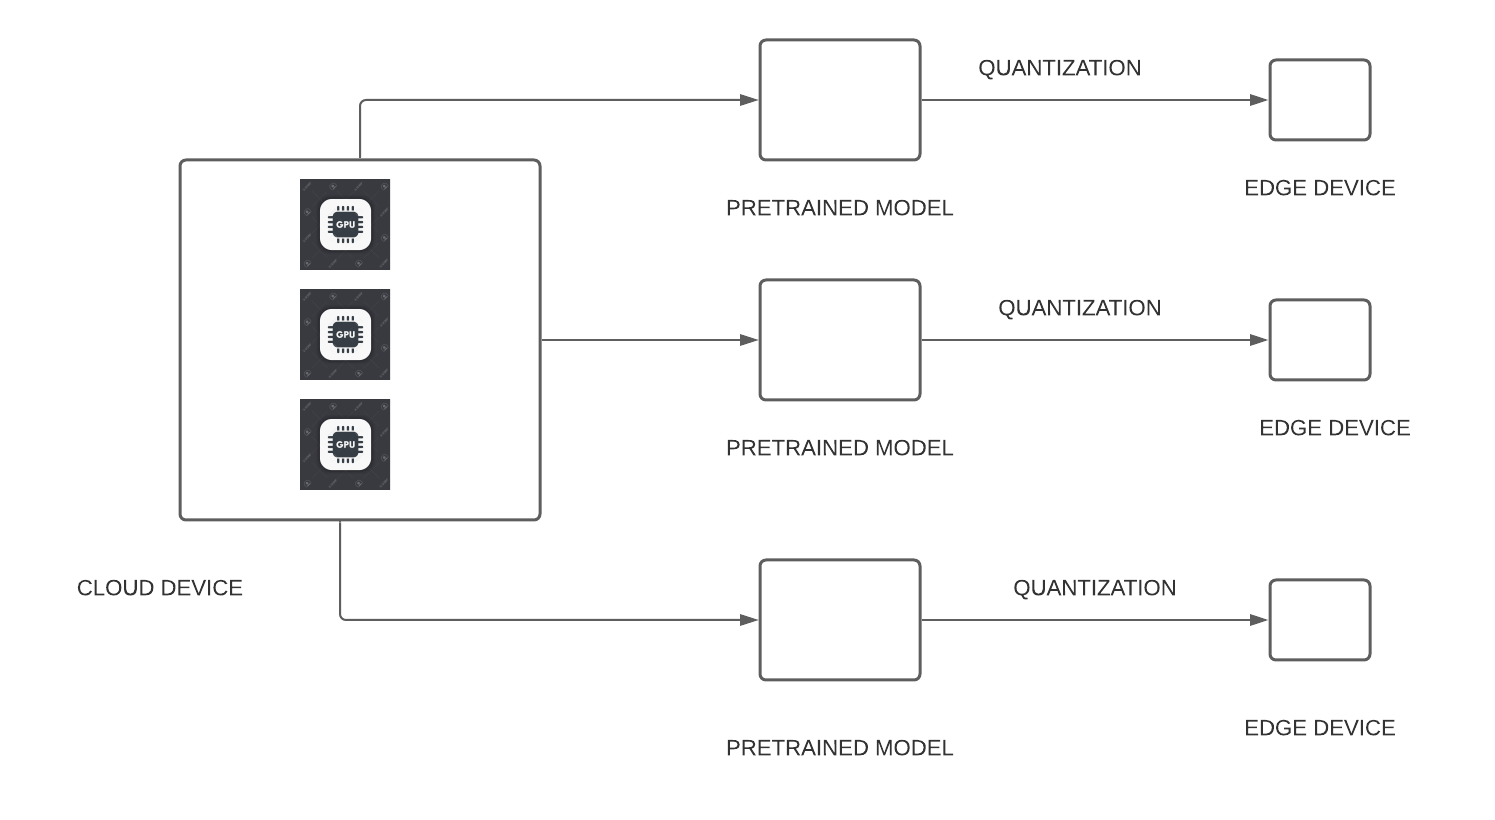
\includegraphics[width=0.5\textwidth]{figures/nmt_edge.png}
\caption{NMT Edge Deployment Framework}
\label{fig:nmtedge}
\end{figure}


\subsection{Model Compression}
The aim of model compression of deep neural networks is to produce a simplified model while not significantly reducing accuracy. The term simplified here refers to a model which has fewer parameters and will use less memory (RAM) during inference. A simplified model is also likely to see a reduction in inference time and lower energy consumption at inference. There are several popular methods of modular compression such as: (i) Pruning, (ii) Quantization, (iii) Low-rank approximation and sparsity, (iv) Knowledge distillation, (v) Neural Architecture Search. 

\subsubsection{Pruning}
Network pruning is essentially the removal of parameters that do not have an impact on network inference accuracy. \cite{pruningandquant} A parameter or neuron may be considered redundant if the coefficients of the weight values are close to zero or exactly zero.

\subsubsection{Knowledge Distillation}
In knowledge distillation (KD) the aim is to produce a simplified model which is able to match the inference accuracy of a more complex model. In KD a larger model is used to train a less computationally complex student network which imitates the functions of the larger model. \cite{pruningandquant}

\subsubsection{Network Architecture Search}
Network architecture search is a method of algorithmically searching for an efficient network from a predetermined search space. 

\subsection{Quantization}
Quantization is the process of approximating a continuous signal by a set of discrete symbols or integer values. \cite{pruningandquant} The goal of model quantization is essentially to reduce the precision of the network components but only to the extent that there is a noticeable reduction in inference time but not in accuracy. 

\subsubsection{Static Quantization}
Static Quantization improves the latency of networks by quantizing the weights ahead of inference. The scale factor and bias for the activation tensors are based on observing the behaviour of the model during a calibration process.

\subsubsection{Dynamic Quantization}
Dyniamic Quantization improves network latency by quantizing the weights before inference, however the activations are dynamically quantized during inference. Dynamic Quantization is more appropriate in situations where the model execution time is dominated by loading weights from memory and not tensor computations. As the NMT model developed consists of two Gated Recurrent Units (GRUs) \cite{gru}, dynamic quantization is more appropriate.

\begin{figure}[t]
\centering
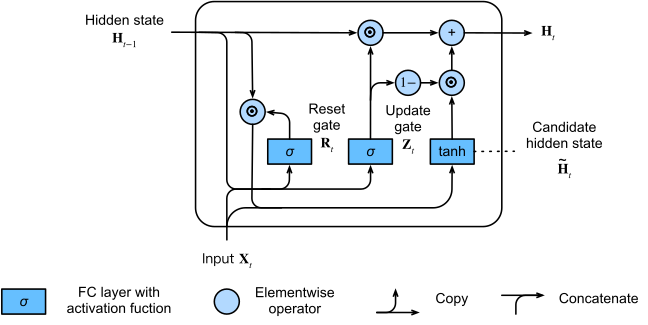
\includegraphics[width=0.5\textwidth]{figures/gru.png}
\caption{Illustration of a Gated Recurrent Unit Cell Architecture \cite{gru} }
\label{fig:grucell}
\end{figure}

\begin{table}[t]
\centering
    \begin{tabular}{ l{1.5cm} l{2.5cm} l{2.5cm} l{1cm} }
     \hline
     Year & Model & \# of Parameters & Dataset Size\\
     \hline
     2019   &   BERT    &   3.4E+08 &   16GB \\
     2019   &   DistillBERT &   6.6E+07 &   16GB \\
     2019 & ALBERT & 2.23E+08 & 16GB \\
     2019 & XLNet (Large) & 3.40 E+08 & 126 GB \\ 
     2020 & ERNIE-GEN (Large) & 3.40 E+08 & 16 GB \\
     2020 & GPT-3 & 1.75E+11 & 570 GB \\
     2021 & Switch-C & 1.57E+12 & 745 GB \\
     \hline
    \end{tabular}
\caption{Overview of Recent Large Language Models \cite{stochasticparrots}}
\label{tab:modeltable}
\end{table}

\section{Neural Translation Model}
Neural Machine Translation consists of utilizing a neural network model to transform a source sentence expressed in one language to a target sentence expressed in a different language. State-of-the-art translation models typically consist of a Sequence-to-Sequence (Seq2Seq) structure. This structure as outlined in \cite{seqtoseq} consists of a (GRU)  cell (see Figure \ref{fig:grucell}) to map the input sequence into a vector. A separate GRU cell is used to decode the target sequence from the encoded vector. To implement the translation model, the steps outlined in the official pytorch tutorial are synthesized. \cite{seq2seqtorch} The specific translation task being performed by the model in this experiment is that of translating an English word, phrase, saying or sentence into its French equivalent.

\subsection{Encoder}
The encoder model is a multi-layer GRU Recurrent Neural Network (RNN) which will take as input a single word from the input sentence. At each time step, the encoder will produce a vector representation for each word as well as a hidden state to be provided as input for the next word in the sequence. The hidden state for the initial token in the sequence is a vector initialized with zeros. For further information on the GRU functionality see Figure \ref{fig:grucell}. The final state output by the encoder is used as the initial hidden state of the decoder. This last output has encoded context from the entire sequence. The encoder architecture is shown in Figure \ref{fig:encoder}.

\begin{figure}[t]
\centering
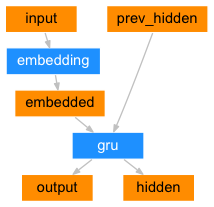
\includegraphics[width=0.25\textwidth]{figures/encoder-network.png}
\caption{Encoder Network Architecture}
\label{fig:encoder}
\end{figure}

\subsection{Decoder}
The decoder takes as input for the first hidden state the final context vector produced from the encoder. The first token used in generating the sequence is the start of sentence '<sos>' token. The global attention mechanism used in \cite{alignandtranslate} is leveraged to focus on salient parts of the input sequence and thus learn the alignment between the segments of the output sequence and their corresponding segments in the input sequence. The decoder's input and hidden state are used to calculate the attention weights for the decoder. These weights are then multiplied by the encoder output vectors to produce a weighted combination. This weighted combination assists the decoder in producing the right output words. The attention mechanism is illustrated in Figure \ref{fig:attention}. To increase the rate at which the model converges, teacher forcing is employed to occasionally directly feed the target outputs as the input at each next time step instead of the decoder's own output. The decoder architecture is shown in Figure \ref{fig:decoder}.

\begin{figure}[t]
\centering
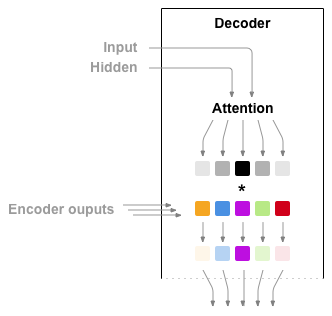
\includegraphics[width=0.4\textwidth]{figures/attention.png}
\caption{Attention Mechanism}
\label{fig:attention}
\end{figure}

\begin{figure}[t]
\centering
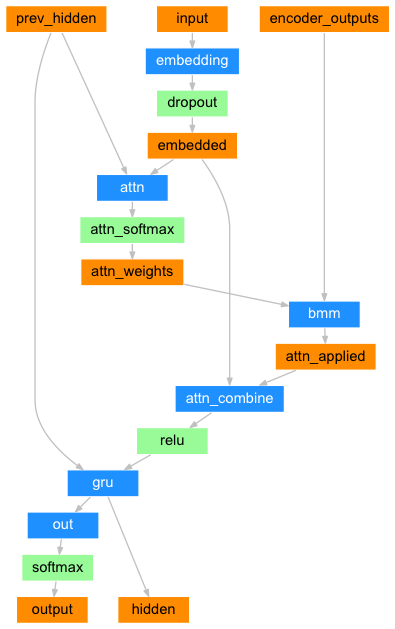
\includegraphics[width=0.35\textwidth]{figures/decoder-network.png}
\caption{Decoder Network Architecture}
\label{fig:decoder}
\end{figure}



\section{Training}
\par The training process used in the official pytorch tutorial, \cite{seq2seqtorch} is replicated here to create the multi-task NMT model outlined in \cite{lowresourcenmtasian}. The dataset used to train the models is taken from the \href{https://en.wikipedia.org/wiki/Tatoeba}{Tatoeba} online repository of example sentences for foreign-language learners. The language pair source sentences and translations are also made \href{https://www.manythings.org/anki/}{available}. Each token in the sentence is replaced with it's index representation in the vocabulary which is manually generated by assigning an integer value to be associated with each token. An end of sentence ('<eos>') token is appended to the sentence before conversion to a tensor. The hidden size of the encoder and decoder is set to 512 and the training process takes place for ~75000 epochs. Model training is done on the publicly available Google Colab GPUs.


\par To track the loss incurred by the encoder in producing the vectorized representation and the decoder in producing the translations, the \href{https://pytorch.org/docs/stable/generated/torch.nn.NLLLoss.html}{Negative Log Likelihood} Loss function is used. This is possible as determining if representations are correct is essentially a classification problem between the representations produced by the model and the labelled output translations. The Stochastic Gradient Descent \cite{sgd} (SGD) Optimization algorithm is utilized for model convergence. A teacher forcing ratio of 0.5 was used to ensure the equal likelihood of the input of the next time step of the decoder being either the true label or the previous decoder output.


\section{Evaluation}
\par The BLEU score \cite{bleu} of the nmt model was evaluated using the available pytorch and nltk libraries.
Formally, the BLEU score is defined by \cite{googlebleu} as: \newline
\begin{math}
BLEU = \underbrace{min (1, exp(1 - \frac{reference\_length}{output\_length}))}_{brevity\ penalty} \underbrace{(\prod_{i = 1}^{4} precision_{i})^{\frac{1}{4}}}_{n-gram\ overlap}
\end{math}

with: \newline

\begin{math}
    precision_{i} = \frac{\sum_{snt \in Cand\-Corpus} \sum_{i \in snt} min (m_{i} cand, m_{i} ref)}{w_{t}^{i} = \sum_{snt^{,} \in Cand\-Corpus} }
\end{math}

where 

\begin{itemize}
  \item m$^{i}_{cand}$ is the count of i-gram in the candidate sentence matching the reference translation.
  
  \item m$^{i}_{ref}$ is the count of i-gram in the reference translation.
  
  \item w$^{i}_{t}$ is the total number of i-grams in candidate translation.
  
  \item The \textbf{Brevity Penalty} penalizes generated translations that are too short compared to the closest reference length.
  
  \item The \textbf{N-Gram Overlap} counts how many n-grams in the candidate match their n-gram counterpart in the reference translation.

\end{itemize}

\par Sample translations from the quantized and original model are shown in table \ref{tab:sample_trans}. In lieu of a holdout dataset for evaluation, the BLEU score of the NMT model on 5000 samples of the corpus of English-French sentence pairs is determined to be approximately 21. When the encoder and decoder models are quantized, there is no reduction in BLEU score. Indicating that satisfactory ML inference can be performed within embedded systems and edge devices.

\begin{table}[t]
\centering
        \textbf{English-French Translations}
    \begin{tabular}{ p{2cm} | p{4cm} }
     \hline
     src & you re temperamental .\\
     \hline
     ref & tu es fantasque .\\
     \hline
     translation & vous etes lunatiques .\\
     \hline
     \hline 
     src & i am afraid to go .\\
     \hline
     ref & j ai peur de m y rendre .\\
     \hline
     translation & j ai peur d y aller .\\
     \hline
     \hline 
     src & you re the oldest .\\
     \hline
     ref & tu es la plus vieille .\\
     \hline
     translation & c est le plus vieux .\\
     \hline
     \hline 
     src & i m surprised you didn t know that .\\
     \hline
     ref & je suis surpris que vous ignoriez cela .\\
     \hline
     translation & je suis surpris que vous ignoriez cela .\\
    \end{tabular}
\caption{Sample Translations}
\label{tab:sample_trans}

\end{table}

\section{Quantization Process}
\par The weight values of the models produced were determined to be approximately 12 MegaBytes (MB) for the encoder and approximately 26 MegaBytes (MB) for the decoder.

\par To reduce the inference time of the neural translation model, dynamic quantization is performed using the \href{https://pytorch.org/docs/stable/quantization.html}{beta-stage pytorch libraries} available. The evaluation results for the quantized and original models can be seen in Table \ref{tab:resultstable}. While the encoder model saw a sizeable reduction in size from 12 MB to 7 MB, there was no reduction in inference accuracy. In the case of the decoder however, the model size was reduced to a half of the original size, also with no loss in inference accuracy.

\begin{table}[t]
\centering
    \begin{tabular}{ |p{2cm}|p{2cm}|}
     \hline
      Bleu Score & Translation Quality\\
     \hline
     <10 & Almost Useless\\
     \hline
     10 - 19 & Hard to get the gist\\
     \hline
     20-29 & Gist is clear w\ Significant Grammatical Errors\\
     \hline
     30 - 40 & Understandable to good translations\\
     \hline
     40-50 & High Quality \\
     \hline
     50 - 60 & Very High Quality, Adequate, Fluent\\
     \hline
     >60 & Better than human \\
     \hline
    \end{tabular}
\caption{Bleu Score Scale}
\label{tab:bleu_score}

\end{table}


\begin{table}[t]

\centering
    \begin{tabular}{ |p{2cm}||p{2cm}|| p{2cm}| }
     \hline
     Model& Size (MB) & BLEU Score\\
     \hline
     Quantized NMT & 7 (Encoder) 13 (Decoder) & 21\\
     \hline
     Original Torch Model & 12 (Encoder) 26 (Decoder) & 21\\
     \hline
    \end{tabular}
\caption{Table Showing BLEU Score for Quantized and original models}
\label{tab:resultstable}

\end{table}

\section{Model Conversion}
\par 


\par The Open Neural Network Exchange (ONNX) standard is an open-source machine independent format that is used for interoperability and exchange between neural network models. \cite{compilingonnx} Pytorch has inherent support for exporting models into the ONNX format and operating them with the ONNX runtime. Unfortunately at the time of this writing, Pytorch does not have support for converting \textbf{quantized} models to ONNX format. 



\section{Code}
The code used in this project can be found in the  \href{https://github.com/dwil2444/NMT_Mobile}{GitHub repository.} The notebook for experiments, code for the Encoder and Decoder GRU models and the weight files for both the original quantized weights are available.

\section{Limitations}
\par The work done in this paper is in response to the actionable recommendations proposed in \cite{energypolicy} to reduce the environmental impact and financial and computational costs associated with NLP model training and inference. A translation model of satisfactory BLEU score was developed and quantized to occupy less memory and reduce inference time, with no loss of accuracy. However due to the lack of support for conversion of quantized models into onnx format, these models could not be converted into various formats, especially those suitable for usage on edge devices and embedded systems. 

\section{Future Work}
\par Extensions for the work done in this paper include incorporating a Federated Learning (FL) framework for ML inferences. Federated learning is a distributed machine learning paradigm introduced by Google which aims to enable edge-devices to collaboratively learn a shared ML model without sharing private or sensitive data. \cite{federated}. Current FL frameworks assume heterogeneity within their respective aggregation schemes, which may be difficult to realise given the varied nature of embedded systems and edge devices. However FL still provides a promising avenue of researching energy efficient deep learning.

\par The development of an Application Programming Interface (API) to support the conversion of Quantized Pytorch models to Open Neural Network Exchange Format is also an avenue for extended work which is being considered. The lack of support for conversion of models from a quantized pytorch framework to an ONNX framework underscores the current underestimation of the need for model efficiency in the ML community.

% \section{Related Work}

% Federated Learning
% Augmented Training

% \section{Acknowledgments}


\bibliographystyle{SIGCHI-Reference-Format}
\bibliography{ref}

\end{document}
